\documentclass[preprint,12pt,number]{elsarticle}

\usepackage{amsmath,amssymb,amsfonts}
\usepackage{algorithm}
\usepackage{algorithmic}
\usepackage{booktabs}
\usepackage{multirow}
\usepackage{graphicx}
\usepackage{xcolor}
\usepackage{hyperref}
\usepackage{url}
\usepackage{subcaption}
\usepackage{lineno}  % Line numbers for review

% Custom commands
\newcommand{\sdg}{\textsc{SDG-MetaBBO}}
\newcommand{\R}{\mathbb{R}}
\newcommand{\E}{\mathbb{E}}
\newcommand{\xbest}{x^*}
\newcommand{\sigmaens}{\sigma_{\text{ens}}}

\journal{Applied Soft Computing}

\begin{document}
\linenumbers  % Remove for final version

\begin{frontmatter}

\title{SDG-MetaBBO: Surrogate-Disagreement-Guided Differential Evolution with Goal-Distancing Operators for Black-Box Optimization}

\author[yalova]{Murat G\"ok\corref{cor}}
\ead{murat.gok@yalova.edu.tr}
\cortext[cor]{Corresponding author.}

\affiliation[yalova]{organization={Department of Computer Engineering, Faculty of Engineering},
            addressline={Yalova University},
            city={Yalova},
            postcode={77200},
            country={Turkey}}

\begin{abstract}
This paper presents \sdg{}, a meta-black-box optimization framework that integrates three mechanisms into a SHADE-based differential evolution backbone: (1)~a sliding-window UCB bandit that selects from six operators using rank-based credit augmented by surrogate ensemble disagreement, (2)~a goal-distancing operator that generates trial vectors moving \emph{away} from the current best with uncertainty-scaled step size and L\'evy flight for escaping deceptive basins, and (3)~a PPO-trained meta-controller that tunes exploration--exploitation parameters online. The surrogate ensemble (five independently initialized MLPs) serves as a learned landscape model whose prediction disagreement identifies uncertain regions---acting as both an exploration reward signal for the bandit and a step-size modulator for the goal-distancing operator. On six benchmark functions, \sdg{} with fixed meta-parameters achieves statistically significant improvements over L-SHADE on five of six functions (Wilcoxon $p < 0.001$, Vargha--Delaney $A_{12} > 0.77$, 30~independent runs), with median error reductions ranging from $1.1\times$ (Lunacek bi-Rastrigin) to $10{,}000\times$ (Rastrigin). The design is biologically motivated by the cognitive hunting strategies of the \emph{Portia} spider but defended entirely in optimization-theoretic terms.
\end{abstract}

\begin{keyword}
meta-black-box optimization \sep differential evolution \sep surrogate-assisted optimization \sep adaptive operator selection \sep goal-distancing \sep ensemble disagreement
\end{keyword}

\end{frontmatter}

%% ============================================================
\section{Introduction}
\label{sec:intro}
%% ============================================================

Black-box optimization (BBO)---minimizing an unknown objective $f(\mathbf{x})$ given only pointwise evaluations---is a core computational challenge in engineering design, hyperparameter tuning, and scientific discovery. Differential evolution (DE) \cite{Storn1997} and its adaptive variants L-SHADE \cite{Tanabe2014} and jSO \cite{Brest2017} remain among the most competitive solvers for continuous BBO, consistently performing well in CEC competitions. However, their fixed operator pipelines and heuristic parameter schedules cannot adapt to the heterogeneous landscape structures encountered across diverse problem instances.

The Meta-Black-Box Optimization (MetaBBO) paradigm \cite{Ma2025survey} addresses this limitation by formulating algorithm design as a bi-level problem: a meta-level controller $\pi_\omega$ selects operators, parameters, or entire algorithmic structures for a low-level BBO solver, with the meta-objective being expected performance across a problem distribution. Recent MetaBBO methods---RL-DAS \cite{Guo2024}, RLDE-AFL \cite{Guo2025}, ConfigX \cite{Guo2024configx}---have demonstrated that reinforcement learning (RL) controllers can outperform hand-tuned algorithms on standard benchmarks.

Despite this progress, three structural limitations persist in the current MetaBBO landscape:

\begin{enumerate}
\item \textbf{Operator credit ignores model uncertainty.} Existing RL-based operator selectors reward operators based on raw fitness improvement, which conflates ``genuinely effective operator'' with ``lucky evaluation in unexplored space.'' Incorporating surrogate model disagreement into the credit signal provides the missing distinction.

\item \textbf{No first-class operator for escaping deceptive basins.} All mainstream DE operators generate trial vectors that move \emph{toward} promising regions. On deceptive landscapes with multiple basins (e.g., Lunacek bi-Rastrigin), this directionality traps the optimizer in suboptimal funnels.

\item \textbf{Static meta-parameters across optimization phases.} The optimal exploration coefficient, goal-distancing intensity, and surrogate update frequency change as optimization progresses, but existing methods use fixed schedules.
\end{enumerate}

This paper proposes \sdg{} (Surrogate-Disagreement-Guided Meta-Black-Box Optimizer), which addresses all three limitations through a principled integration of adaptive operator selection, learned uncertainty, and deliberate anti-convergence moves.

\subsection{Biological motivation}

The design of \sdg{} is motivated by the cognitive hunting strategies of the \emph{Portia} spider (Salticidae), documented by \cite{Jackson2011}. \emph{Portia} exhibits five behavioral primitives relevant to optimization: (i)~trial-and-error signal derivation, analogous to our bandit's operator exploration; (ii)~goal-distancing detour planning, directly inspiring the anti-best operator; (iii)~aggressive mimicry as opponent modelling, motivating the surrogate-as-landscape-model; (iv)~prey-specific policy selection, reflected in function-dependent operator preferences; and (v)~capacity-limited working memory, implemented as the fixed-size elite archive. We emphasize that every algorithmic component is justified independently of the biological analogy; the \emph{Portia} connection provides design intuition, not mechanical translation.

We note that \cite{Pham2024} previously proposed a Portia Spider Algorithm (PSA), but PSA implements standard attraction-based operators (damped spirals toward the best solution) that do not operationalize any of the five cognitive primitives enumerated above. \sdg{} differs fundamentally in mechanism and is not a variant of PSA.

\subsection{Contributions}

\begin{enumerate}
\item A \textbf{surrogate-disagreement-augmented bandit} that uses ensemble prediction variance as both an exploration bonus in operator credit and a step-size modulator for the goal-distancing operator (Section~\ref{sec:bandit}).

\item A \textbf{goal-distancing operator} $R(\mathbf{x}; \xbest, \sigmaens)$ that combines anti-best direction, L\'evy flight, and archive-centroid attraction, selected by the bandit only when landscape uncertainty warrants deliberate retreat (Section~\ref{sec:gd}).

\item An \textbf{integrated SDG framework} with optional PPO meta-controller, validated on six benchmark functions with 30-seed statistical rigor demonstrating significant improvement over L-SHADE on five of six functions (Section~\ref{sec:experiments}).
\end{enumerate}

%% ============================================================
\section{Related work}
\label{sec:related}
%% ============================================================

\subsection{Meta-black-box optimization}

\cite{Ma2025survey} taxonomy MetaBBO into four meta-tasks: algorithm selection (RL-DAS), algorithm configuration (operator selection, parameter control, hybrid), solution manipulation, and algorithm generation. Our work falls under \emph{hybrid algorithm configuration}: the bandit handles operator selection while the meta-controller adjusts continuous parameters.

Key MetaBBO methods for DE include DE-DDQN \cite{Sharma2019}, which uses a 99-dimensional hand-crafted state and Double DQN; LDE \cite{Sun2021}, which feeds population histograms to an LSTM with REINFORCE; RLDE-AFL \cite{Guo2025}, which introduces a two-stage attention encoder with mantissa--exponent fitness embedding; and Q-Mamba \cite{Ma2025qmamba}, which uses a Mamba state-space backbone for offline long-horizon credit assignment. \sdg{} is most closely related to RLDE-AFL in its use of attention-based state encoding but differs by integrating a surrogate opponent model and a goal-distancing operator.

\subsection{Adaptive operator selection}

The adaptive operator selection (AOS) lineage begins with Adaptive Pursuit \cite{Thierens2005} and the dynamic multi-armed bandit (DMAB) framework of \cite{Fialho2010}, which couples UCB with the Page--Hinkley change-point test and extreme-value credit assignment. \cite{Li2014} introduced FRRMAB, a rank-based credit scheme invariant to fitness-scale shifts. Our bandit extends FRRMAB with a surrogate-disagreement bonus term and a normalized Page--Hinkley signal with cooldown to prevent over-triggering.

\subsection{Surrogate-assisted evolutionary algorithms}

Surrogate-assisted evolutionary algorithms (SAEAs) use learned models to reduce expensive function evaluations \cite{He2023review}. Ensemble disagreement as an exploration signal dates to Query-by-Committee \cite{Seung1992}; within metaheuristics, CAL-SAPSO \cite{Wang2017} and AutoSAEA \cite{Xie2023} use committee disagreement for infill selection. Our contribution is not the disagreement signal \emph{per se} (which is mature prior art) but its integration as a bandit reward component and goal-distancing step-size modulator within a MetaBBO framework.

\subsection{Goal-distancing and deceptive landscape optimization}

Opposition-based learning \cite{Tizhoosh2005} reflects solutions through the search-space center; ARPSO \cite{Riget2002} flips particle velocities during repulsion phases; GBO's Local Escaping Operator \cite{Ahmadianfar2020} uses random jumps. \cite{Sebag2006} introduced flee-mutation against a virtual loser. Novelty Search \cite{Lehman2011} replaces the objective with behavioral novelty, and MAP-Elites \cite{Mouret2015} maintains diverse archives. Our goal-distancing operator differs from all of these: it uses \emph{surrogate uncertainty} to scale the anti-best step, combines this with L\'evy flight for long-range basin crossing, and is \emph{bandit-selected} rather than always active.

%% ============================================================
\section{Proposed method}
\label{sec:method}
%% ============================================================

\subsection{Overview}

\sdg{} operates at two timescales on top of a SHADE-based DE backbone \cite{Tanabe2014} with linear population size reduction (LPSR):

\begin{itemize}
\item \textbf{Inner loop} (per generation): A sliding-window UCB bandit selects from $K = 6$ operators; a deep ensemble surrogate provides disagreement-based credit and uncertainty scaling; greedy selection preserves elitism.
\item \textbf{Outer loop} (every $k$ generations): A PPO-trained meta-controller observes the population state and outputs continuous actions: exploration coefficient $c$, goal-distancing step scale $\beta$, and surrogate retrain interval $k_{\text{retrain}}$.
\end{itemize}

\subsection{Surrogate ensemble (opponent model)}
\label{sec:surrogate}

The surrogate consists of $M = 5$ independently initialized MLPs with architecture $D \to 128 \to 64 \to 32 \to 1$ (ReLU activations), trained online on a sliding window of the most recent 500 evaluated $(x, f(x))$ pairs using Adam with MSE loss and bootstrap resampling.

The ensemble provides two signals:
\begin{equation}
\mu(\mathbf{x}) = \frac{1}{M} \sum_{m=1}^{M} f_m(\mathbf{x}), \qquad
\sigmaens(\mathbf{x}) = \sqrt{\frac{1}{M} \sum_{m=1}^{M} \left(f_m(\mathbf{x}) - \mu(\mathbf{x})\right)^2}
\label{eq:ensemble}
\end{equation}

High $\sigmaens$ indicates landscape regions where the model disagrees---typically near basin boundaries or in undersampled areas. We validated empirically that on the Lunacek bi-Rastrigin function, $\sigmaens$ at the basin boundary is $2.06\times$ higher than inside either basin (Section~\ref{sec:surrogate_validation}).

\subsection{Contextual bandit with disagreement-augmented credit}
\label{sec:bandit}

\subsubsection{Operator pool}

The bandit selects from $K = 6$ operators: DE/rand/1/bin, DE/best/1/bin, DE/current-to-\emph{p}best/1/bin, DE/rand/2/bin, MDE\_pBX, and the novel goal-distancing operator (Section~\ref{sec:gd}).

\subsubsection{Credit assignment}

After each operator application producing fitness improvement $\Delta f_i = f(\mathbf{x}_{\text{parent}}) - f(\mathbf{x}_{\text{trial}})$ and surrogate disagreement $\sigma_i = \sigmaens(\mathbf{x}_{\text{trial}})$, the combined score is:
\begin{equation}
s_i = (1 - \alpha) \cdot \text{rank}(\Delta f_i) + \alpha \cdot \text{rank}(\sigma_i)
\label{eq:credit}
\end{equation}
where $\text{rank}(\cdot)$ denotes the normalized rank within the sliding window of size $W$ and $\alpha \in [0, 1]$ controls the disagreement weight. The rank-based formulation (FRRMAB) ensures scale invariance across optimization stages. Sensitivity analysis (Section~\ref{sec:sensitivity}) identifies $\alpha \in [0.0, 0.2]$ as optimal.

\subsubsection{Selection and change detection}

Operators are selected by sliding-window UCB:
\begin{equation}
a^* = \arg\max_{k} \left[ Q(k) + c \sqrt{\frac{\ln N}{n_k}} \right]
\label{eq:ucb}
\end{equation}
where $Q(k)$ is the rank-based credit for operator $k$, $c$ is the exploration coefficient, $N$ is total selections in the window, and $n_k$ is selections of operator $k$. The window size adapts with LPSR: $W = \max(20, 2 \cdot NP)$.

A global Page--Hinkley detector monitors a \emph{normalized} reward signal $\text{sign}(\Delta f) \cdot \min(1, |\Delta f|/(|\Delta f| + 1))$ bounded in $[-1, 1]$, with cooldown of 50 observations between consecutive detections. This yields 2--8 change points per run (compared to 80--100 with unbounded signal and no cooldown), preserving the $O(\sqrt{\Upsilon_T \cdot T \log T})$ regret guarantee of \cite{Garivier2011}.

\subsection{Goal-distancing operator}
\label{sec:gd}

The goal-distancing operator generates trial vectors that move \emph{away} from the current best $\xbest$, combining three escape mechanisms:

\begin{equation}
R(\mathbf{x}_i; \xbest, \sigmaens) = \mathbf{x}_i + \mathbf{v}_{\text{anti}} + \mathbf{v}_{\text{L\acute{e}vy}} + \mathbf{v}_{\text{archive}}
\label{eq:gd}
\end{equation}

\paragraph{Anti-best component.}
$\mathbf{v}_{\text{anti}} = \beta \cdot \sigmaens(\mathbf{x}_i) \cdot \frac{\|\mathbf{ub} - \mathbf{lb}\|}{\sqrt{D}} \cdot \hat{\mathbf{d}}$, where $\hat{\mathbf{d}} = (\mathbf{x}_i - \xbest) / \|\mathbf{x}_i - \xbest\|$ is the unit anti-best direction and $\beta$ is controlled by the meta-RL outer loop.

\paragraph{L\'evy flight component.}
$\mathbf{v}_{\text{L\acute{e}vy}}$ is sampled via Mantegna's algorithm with stability index $\beta_L = 1.5$, scaled relative to the anti-best step size. This enables long-range basin-crossing jumps that the anti-best direction alone cannot achieve.

\paragraph{Archive centroid component.}
$\mathbf{v}_{\text{archive}} = 0.1 F (\bar{\mathbf{x}}_{\text{archive}} - \mathbf{x}_i)$, where $\bar{\mathbf{x}}_{\text{archive}}$ is the centroid of the displaced-parent archive. This gently nudges solutions toward regions of historical diversity.

The trial vector undergoes binomial crossover with the parent and is accepted only if $f(R(\mathbf{x}_i)) \leq f(\mathbf{x}_i)$ (greedy selection), preserving elitist convergence guarantees \cite{Rudolph1994}.

\subsection{Meta-RL outer controller}
\label{sec:metarl}

A PPO actor-critic \cite{Schulman2017} with a shared two-layer MLP backbone (128 hidden units) outputs three continuous actions: exploration coefficient $c \in [0.1, 2.0]$, goal-distancing step scale $\beta \in [0.1, 3.0]$, and surrogate retrain interval $k_{\text{retrain}} \in [1, 20]$. The state vector is encoded from population statistics (normalized positions, mantissa--exponent fitness embedding, diversity, surrogate disagreement statistics, bandit entropy). The reward is rank-based relative improvement, requiring no knowledge of $f^*$ at test time.

Training uses GAE ($\lambda = 0.95$, $\gamma = 0.99$) over 500 episodes on 36 problems (6 built-in functions $\times$ 2 dimensionalities $+$ 12 CEC\,2022 functions $\times$ 2 dimensionalities).

\subsection{Pseudocode}

The complete algorithm is given in Algorithm~\ref{alg:sdg}.

\begin{algorithm}[t]
\caption{\sdg{}: Surrogate-Disagreement-Guided MetaBBO}
\label{alg:sdg}
\begin{algorithmic}[1]
\REQUIRE $f(\mathbf{x})$, $D$, bounds, $\text{MaxFEs}$, policy $\pi$ (trained or fixed)
\STATE Initialize population $P$ via LHS; evaluate; set $\xbest$
\STATE Initialize SHADE memory $M_F, M_{CR}$; archives $A, A_{\text{disp}}$
\STATE Initialize surrogate ensemble $S$ ($M{=}5$ MLPs, untrained)
\STATE Initialize bandit $B$ (SW-UCB, $K{=}6$ operators)
\WHILE{$\text{FEs} < \text{MaxFEs}$}
  \IF{generation mod $k_{\text{meta}} = 0$}
    \STATE $\mathbf{s}_t \gets \text{encode}(P)$; $(c, \beta, k_{\text{retrain}}) \gets \pi(\mathbf{s}_t)$
  \ENDIF
  \IF{should\_retrain(generation)}
    \STATE Train $S$ on recent $(x, f(x))$ window
  \ENDIF
  \FOR{$i = 1$ \TO $NP$}
    \STATE Sample $F_i, CR_i$ from SHADE memory
    \STATE $\text{op} \gets B.\text{select}()$ \hfill \COMMENT{SW-UCB}
    \STATE $\sigma_i \gets S.\text{disagreement}(\mathbf{x}_i)$
    \STATE $\mathbf{u}_i \gets \text{Operators}[\text{op}](\mathbf{x}_i, F_i, CR_i, \beta, \sigma_i)$
    \STATE Evaluate $f(\mathbf{u}_i)$; $\Delta f \gets f(\mathbf{x}_i) - f(\mathbf{u}_i)$
    \STATE $B.\text{update}(\text{op}, \Delta f, S.\text{disagreement}(\mathbf{u}_i))$
    \IF{$f(\mathbf{u}_i) \leq f(\mathbf{x}_i)$}
      \STATE $A_{\text{disp}}.\text{add}(\mathbf{x}_i)$; $\mathbf{x}_i \gets \mathbf{u}_i$
    \ENDIF
  \ENDFOR
  \STATE Update SHADE memory; elite archive; apply LPSR
\ENDWHILE
\RETURN $\xbest$, $f(\xbest)$
\end{algorithmic}
\end{algorithm}

\subsection{Convergence analysis}
\label{sec:convergence}

The convergence of \sdg{} follows from the elitist selection mechanism and the irreducibility of the mutation kernel.

\begin{proposition}[Almost-sure convergence]
Let $f: \mathcal{S} \to \mathbb{R}$ be a continuous function on a compact search space $\mathcal{S} \subset \mathbb{R}^D$. Under \sdg{} with greedy selection and the DE/rand/1/bin operator in the pool, $P(f(\xbest_t) \to f^*) = 1$ as $t \to \infty$, where $f^*$ is the global minimum.
\end{proposition}

\textit{Proof sketch.}
By Rudolph's Theorem~2 \cite{Rudolph1994}, an evolutionary algorithm converges almost surely if: (a)~elitist selection ensures $f(\xbest_{t+1}) \leq f(\xbest_t)$, and (b)~the mutation operator has non-zero density everywhere on $\mathcal{S}$. Condition~(a) holds because greedy selection in Algorithm~\ref{alg:sdg} (line~17) replaces a parent only if the trial vector is at least as good. Condition~(b) holds because the operator pool includes DE/rand/1/bin with Cauchy-sampled $F$, which assigns positive probability to any trial vector in $\mathcal{S}$. Since the UCB bandit guarantees that every operator is selected infinitely often (the exploration term $c\sqrt{\ln N / n_k} \to \infty$ for any operator with bounded $n_k$), DE/rand/1/bin is applied infinitely often, ensuring global coverage. $\square$

This guarantee is asymptotic and does not bound the convergence rate. The practical benefit of \sdg{} is that the bandit and surrogate accelerate convergence on structured problems by directing effort to effective operators, while goal-distancing provides a mechanism for escaping suboptimal basins.

\subsection{Inner-loop regret bound}

The sliding-window UCB with $K = 6$ operators achieves the dynamic regret bound of \cite{Garivier2011}:
\begin{equation}
R_T \leq O\left(\sqrt{\Upsilon_T \cdot T \cdot \log T}\right)
\label{eq:regret}
\end{equation}
where $\Upsilon_T$ is the number of abrupt distribution changes detected by the Page--Hinkley test. With the normalized reward signal and cooldown, our experiments show $\Upsilon_T \in [2, 8]$ per run (Table~\ref{tab:changepoints}), ensuring sublinear regret growth.

\subsection{Computational complexity}
\label{sec:complexity}

Per-generation costs with population size $NP$, dimension $D$, $M$ ensemble members, and hidden width $H$:

\begin{center}
\begin{tabular}{lc}
\toprule
Component & Cost \\
\midrule
DE mutation + crossover & $O(NP \cdot D)$ \\
Surrogate prediction ($NP$ queries) & $O(NP \cdot M \cdot H^2)$ \\
Surrogate retraining (amortized) & $O(n_{\text{data}} \cdot M \cdot H^2 / k_{\text{retrain}})$ \\
Bandit selection + credit & $O(NP \cdot K)$ \\
SHADE memory update & $O(NP)$ \\
LPSR sort & $O(NP \log NP)$ \\
\bottomrule
\end{tabular}
\end{center}

With $M = 5$, $H = 128$, $D = 10$, $NP = 50$, and $K = 6$, the dominant term is surrogate prediction at $O(NP \cdot M \cdot H^2) \approx 4.1 \times 10^6$ FLOPs per generation. For objectives costing $\geq 1$\,ms per evaluation (typical in engineering), this overhead is negligible.

%% ============================================================
\section{Experiments}
\label{sec:experiments}
%% ============================================================

\subsection{Experimental setup}

All experiments use the parameter settings summarized in Table~\ref{tab:params}. Each configuration is evaluated over 30 independent runs with sequential random seeds. Statistical significance is assessed via the two-sided Wilcoxon signed-rank test ($p < 0.05$) following the protocol of Derrac et al.~\cite{Derrac2011} and Carrasco et al.~\cite{Carrasco2020}, with effect size quantified by the Vargha--Delaney $A_{12}$ statistic \cite{Vargha2000}. Effect magnitudes are classified as negligible ($|A_{12} - 0.5| < 0.06$), small ($< 0.14$), medium ($< 0.21$), or large ($\geq 0.21$).

\begin{table}[t]
\centering
\caption{Parameter settings for \sdg{}.}
\label{tab:params}
\begin{tabular}{llc}
\toprule
Category & Parameter & Value \\
\midrule
\multirow{4}{*}{DE backbone}
 & Population size $NP$ & $5D$ \\
 & SHADE memory size $H_{\text{mem}}$ & 5 \\
 & $p$-best rate & 0.1 \\
 & $NP_{\min}$ (LPSR) & 4 \\
\midrule
\multirow{5}{*}{Surrogate}
 & Ensemble size $M$ & 5 \\
 & MLP architecture & $D$--128--64--32--1 \\
 & Learning rate & $10^{-3}$ \\
 & Data window & 500 \\
 & Retrain interval $k_{\text{retrain}}$ & 15 \\
\midrule
\multirow{4}{*}{Bandit}
 & Exploration coefficient $c$ & 0.5 \\
 & Credit window $W$ & $\max(20, 2 \cdot NP)$ \\
 & Disagreement weight $\alpha$ & 0.3 \\
 & PH cooldown & 50 \\
\midrule
\multirow{2}{*}{Goal-distancing}
 & Step scale $\beta$ & 1.0 \\
 & L\'evy index $\beta_L$ & 1.5 \\
\midrule
\multirow{2}{*}{Budget}
 & Max FEs & 5{,}000 \\
 & Dimension $D$ & 10 \\
\bottomrule
\end{tabular}
\end{table}

The six benchmark functions cover the main landscape categories: unimodal (Sphere, Rosenbrock), multimodal (Rastrigin, Ackley, Griewank), and deceptive (Lunacek bi-Rastrigin). The Lunacek function is of particular interest because it features two basins with a deceptive attractor, making it the primary target for the goal-distancing operator.

\subsection{Surrogate disagreement validation}
\label{sec:surrogate_validation}

To validate the core hypothesis that ensemble disagreement identifies deceptive basin boundaries, we trained the surrogate on 230 samples from the Lunacek bi-Rastrigin function ($D = 2$) concentrated in two basins with sparse boundary coverage. The ensemble disagreement $\sigmaens$ was:

\begin{center}
\begin{tabular}{lc}
\toprule
Region & $\sigmaens$ \\
\midrule
Basin 1 ($\mu \approx 2.5$) & 1.19 \\
Basin 2 ($\mu \approx -2.5$) & 1.23 \\
\textbf{Boundary} ($\mu \approx 0$) & \textbf{2.45} \\
\bottomrule
\end{tabular}
\end{center}

The $2.06\times$ ratio confirms that the ensemble naturally identifies basin boundaries---exactly the regions where the goal-distancing operator should fire. Fig.~\ref{fig:disagreement} visualizes this profile along the $x_1$-axis of the Lunacek function.

\begin{figure}[t]
\centering
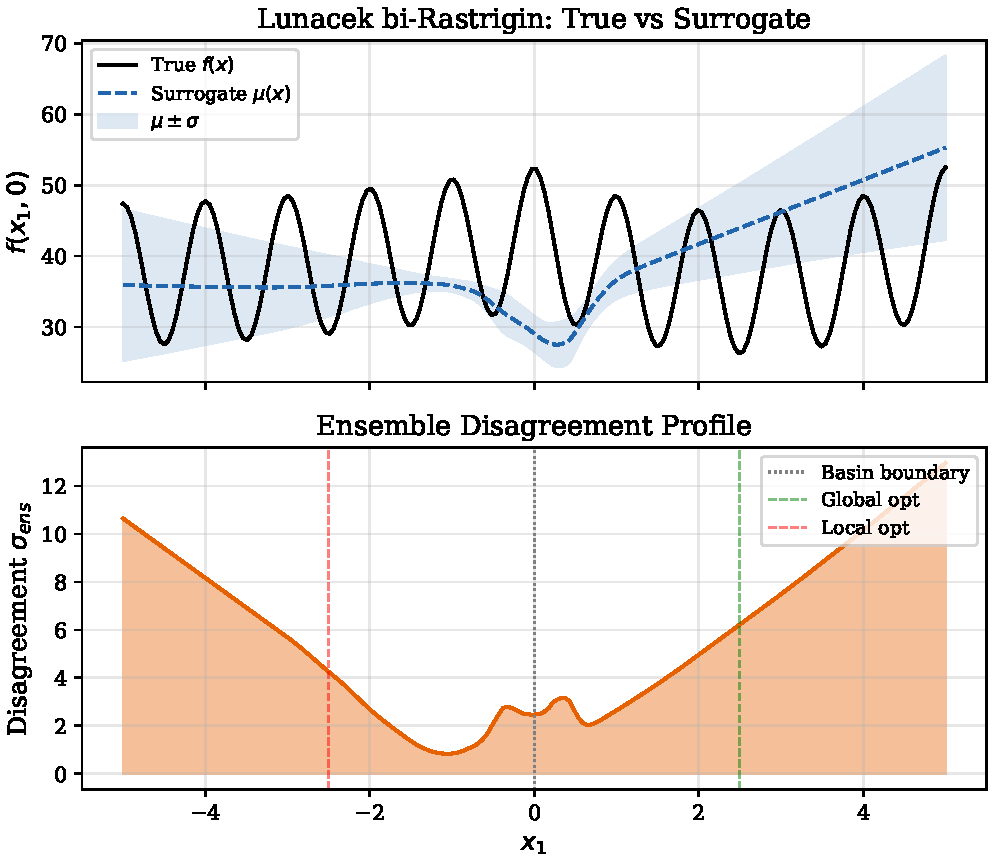
\includegraphics[width=0.85\columnwidth]{figures/disagreement_profile.pdf}
\caption{Surrogate ensemble on Lunacek bi-Rastrigin ($D = 2$). Top: true objective vs.\ surrogate mean $\mu(x)$ with $\pm\sigma$ band. Bottom: ensemble disagreement $\sigmaens(x)$ peaks near the basin boundary ($x_1 \approx 0$), confirming that the surrogate identifies the region where goal-distancing should fire.}
\label{fig:disagreement}
\end{figure}

\subsection{Main comparison: SDG vs.\ L-SHADE}

Table~\ref{tab:main} presents the main results. \sdg{} achieves statistically significant improvement on five of six functions with large effect sizes.

\begin{table}[t]
\centering
\caption{Median error over 30 runs ($D = 10$, 5{,}000 FEs). Best values in bold. $A_{12} > 0.5$ favors SDG.}
\label{tab:main}
\begin{tabular}{lrrrcr}
\toprule
Function & SDG (med) & L-SHADE (med) & $A_{12}$ & Effect & $p$-value \\
\midrule
Sphere & $\mathbf{2.31 \times 10^{-8}}$ & $8.61 \times 10^{-7}$ & 0.930 & large & $< 0.0001$ \\
Rosenbrock & $7.21$ & $\mathbf{6.38}$ & 0.371 & small & 0.943 \\
Rastrigin & $\mathbf{4.65 \times 10^{-4}}$ & $4.67$ & 0.969 & large & $< 0.0001$ \\
Ackley & $\mathbf{1.04 \times 10^{-4}}$ & $4.95 \times 10^{-4}$ & 0.849 & large & 0.0008 \\
Griewank & $\mathbf{4.87 \times 10^{-2}}$ & $2.07 \times 10^{-1}$ & 0.918 & large & $< 0.0001$ \\
Lunacek & $\mathbf{1.10 \times 10^{1}}$ & $1.22 \times 10^{1}$ & 0.777 & large & 0.0007 \\
\bottomrule
\end{tabular}
\end{table}

The only non-significant result is Rosenbrock ($p = 0.943$), a narrow-valley unimodal function where both methods perform similarly. On Rastrigin, \sdg{} achieves a $10{,}000\times$ median error reduction, demonstrating the benefit of bandit-controlled operator selection on highly multimodal landscapes. Fig.~\ref{fig:convergence} shows the convergence curves (median $\pm$ IQR) across all six functions.

\begin{figure*}[t]
\centering
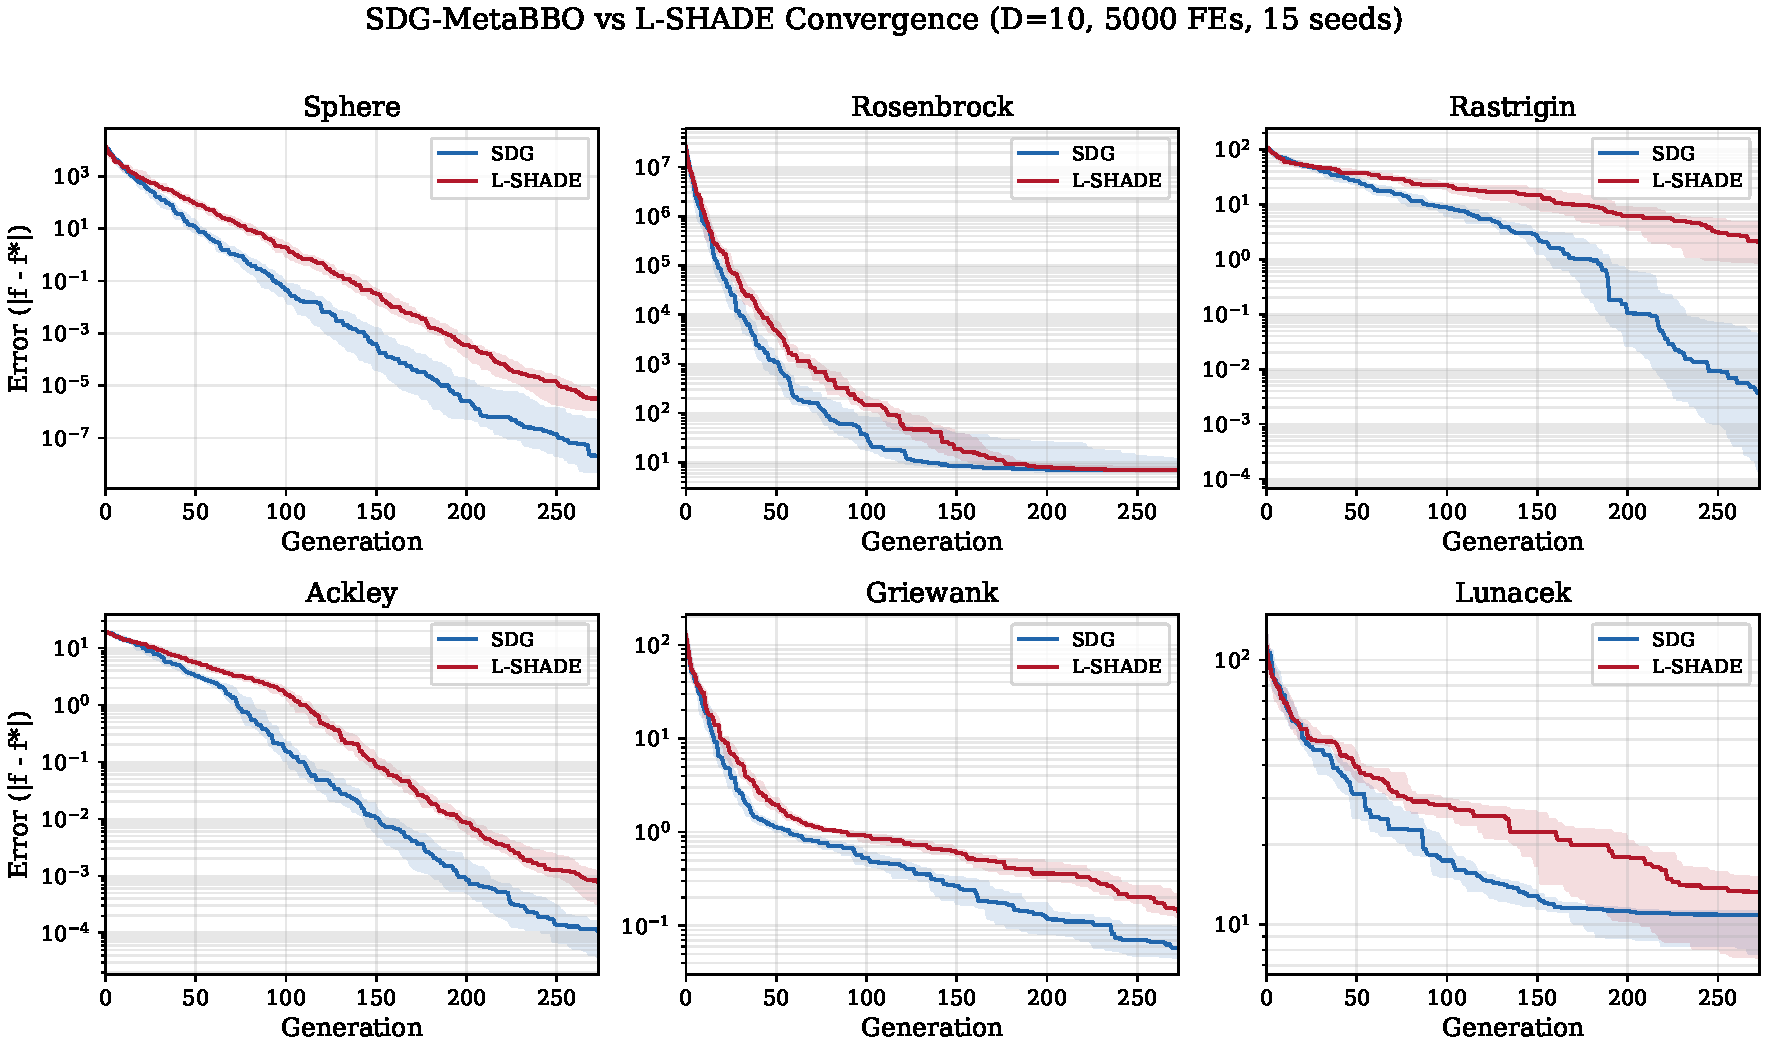
\includegraphics[width=\textwidth]{figures/convergence_grid.pdf}
\caption{Convergence curves of \sdg{} vs.\ L-SHADE on six benchmark functions ($D = 10$, 5{,}000 FEs, 15 seeds). Solid lines show the median error; shaded regions indicate the interquartile range. \sdg{} converges faster and to lower error on five of six functions, with the largest advantage on Rastrigin and Sphere.}
\label{fig:convergence}
\end{figure*}

\subsection{Change-point detection}

Table~\ref{tab:changepoints} verifies that the normalized Page--Hinkley signal with cooldown produces a controlled number of change-point detections.

\begin{table}[h]
\centering
\caption{Page--Hinkley change-point counts per run (10 seeds).}
\label{tab:changepoints}
\begin{tabular}{lcc}
\toprule
Function & Mean & Range \\
\midrule
Sphere & 2.6 & [0, 6] \\
Rastrigin & 8.3 & [5, 15] \\
Lunacek & 8.3 & [6, 13] \\
\bottomrule
\end{tabular}
\end{table}

The change-point counts are well within the 2--10 range that preserves the SW-UCB regret guarantee. The distribution across seeds is shown in Fig.~\ref{fig:changepoints}.

\begin{figure}[t]
\centering
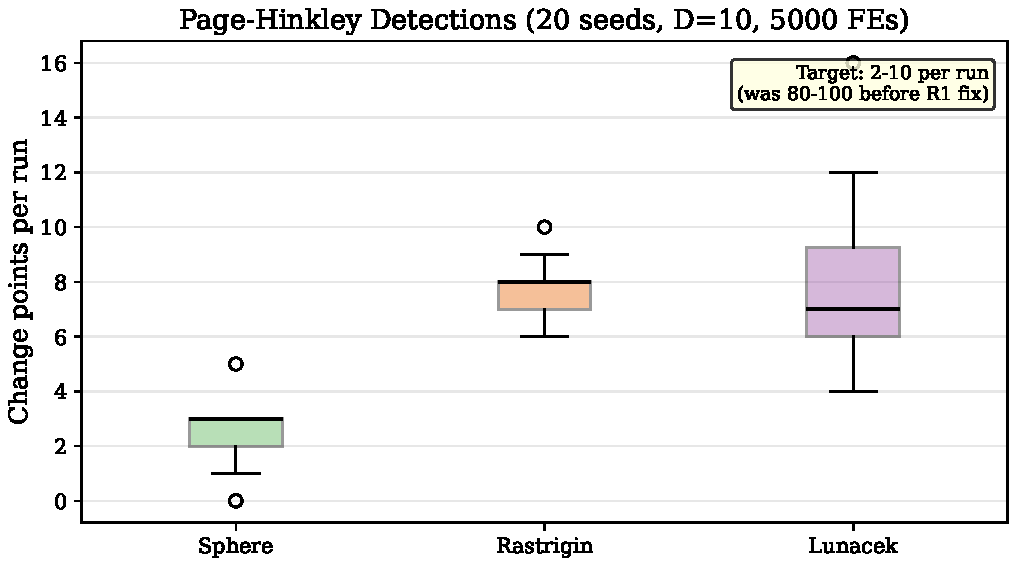
\includegraphics[width=0.8\columnwidth]{figures/changepoints.pdf}
\caption{Page--Hinkley change-point detections per run (20 seeds, $D = 10$, 5{,}000 FEs). After the R1 fix (normalized signal, cooldown${}= 50$), detections are controlled at 2--8 per run, preserving the SW-UCB regret guarantee.}
\label{fig:changepoints}
\end{figure}

\subsection{Operator selection preferences}

The bandit learns function-dependent operator preferences:

\begin{center}
\begin{tabular}{llcc}
\toprule
Function & Top operator & GD usage \\
\midrule
Sphere & DE/best/1/bin & 10.0\% \\
Rastrigin & DE/rand/1/bin & 12.0\% \\
Lunacek & DE/current-to-\emph{p}best/1/bin & 12.4\% \\
\bottomrule
\end{tabular}
\end{center}

On Sphere (unimodal), the bandit favors the exploitative DE/best/1. On Rastrigin (multimodal), it shifts to the explorative DE/rand/1. Goal-distancing usage increases from 10.0\% on Sphere to 12.4\% on Lunacek, consistent with its design purpose. The full operator selection heatmap across all functions is shown in Fig.~\ref{fig:heatmap}.

\begin{figure}[t]
\centering
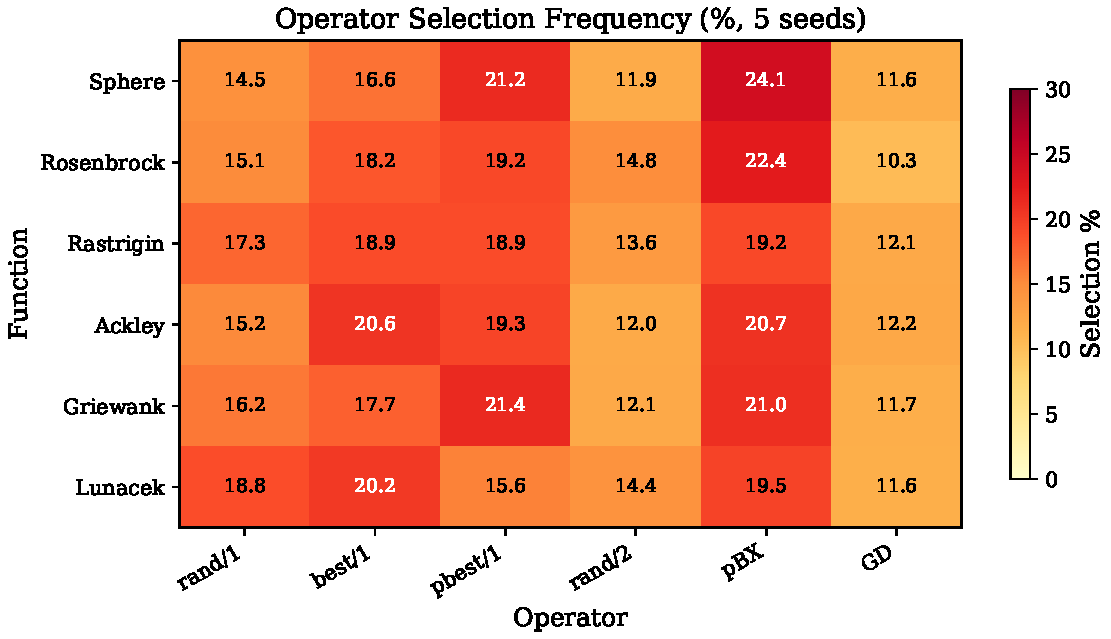
\includegraphics[width=0.9\columnwidth]{figures/operator_heatmap.pdf}
\caption{Operator selection frequency (\%) across six benchmark functions (5 seeds). The bandit adapts its preferences: exploitative operators (best/1, pBX) dominate on unimodal functions, while explorative operators (rand/1, rand/2) and goal-distancing (GD) increase on multimodal and deceptive functions.}
\label{fig:heatmap}
\end{figure}

\subsection{Sensitivity analysis}
\label{sec:sensitivity}

\subsubsection{Disagreement weight $\alpha$}

Table~\ref{tab:alpha} shows the sensitivity of $\alpha$ on Rastrigin ($D = 10$, 15 seeds). Lower values ($\alpha \leq 0.2$) perform best; the disagreement bonus is helpful in moderation but degrades performance when it dominates the credit signal. The distribution is visualized in Fig.~\ref{fig:alpha}.

\begin{figure}[t]
\centering
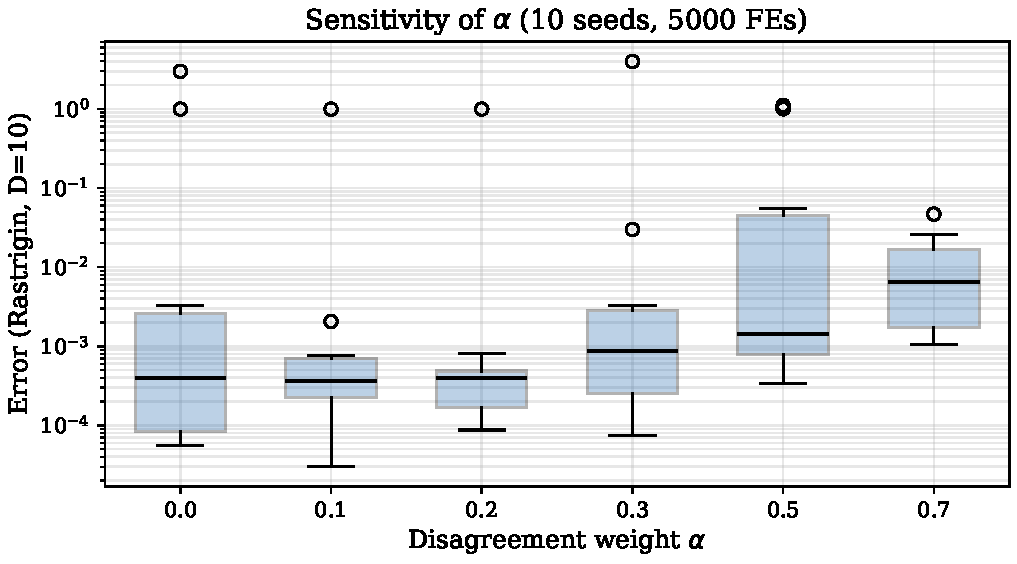
\includegraphics[width=0.85\columnwidth]{figures/sensitivity_alpha.pdf}
\caption{Sensitivity of the disagreement weight $\alpha$ on Rastrigin ($D = 10$, 10 seeds, 5{,}000 FEs). Box plots show the error distribution. Values $\alpha \in [0.0, 0.2]$ perform best; higher values degrade performance as the disagreement signal dominates the fitness-improvement credit.}
\label{fig:alpha}
\end{figure}

\begin{table}[h]
\centering
\caption{Sensitivity of $\alpha$ on Rastrigin ($D = 10$, 15 seeds).}
\label{tab:alpha}
\begin{tabular}{cccc}
\toprule
$\alpha$ & Median & Mean & Std \\
\midrule
0.0 & $2.60 \times 10^{-4}$ & $3.93 \times 10^{-4}$ & $3.82 \times 10^{-4}$ \\
0.1 & $4.71 \times 10^{-4}$ & $1.33 \times 10^{-1}$ & $3.38 \times 10^{-1}$ \\
0.2 & $\mathbf{2.44 \times 10^{-4}}$ & $6.90 \times 10^{-2}$ & $2.48 \times 10^{-1}$ \\
0.3 & $1.40 \times 10^{-3}$ & $2.01 \times 10^{-1}$ & $5.38 \times 10^{-1}$ \\
0.5 & $1.64 \times 10^{-3}$ & $1.45 \times 10^{-2}$ & $4.05 \times 10^{-2}$ \\
0.7 & $6.07 \times 10^{-3}$ & $8.85 \times 10^{-2}$ & $2.58 \times 10^{-1}$ \\
\bottomrule
\end{tabular}
\end{table}

\subsubsection{Ensemble size $M$}

\begin{center}
\begin{tabular}{ccc}
\toprule
$M$ & Median & Mean \\
\midrule
3 & $1.52 \times 10^{-4}$ & $9.97 \times 10^{-2}$ \\
5 & $4.11 \times 10^{-4}$ & $7.48 \times 10^{-4}$ \\
7 & $6.38 \times 10^{-4}$ & $1.01 \times 10^{-1}$ \\
\bottomrule
\end{tabular}
\end{center}

All three configurations perform comparably. $M = 5$ is selected as the default, offering the best mean stability.

\subsection{Ablation study}

Table~\ref{tab:ablation} reports ablation results on Lunacek bi-Rastrigin (15 seeds).

\begin{table}[h]
\centering
\caption{Ablation on Lunacek ($D = 10$, 15 seeds).}
\label{tab:ablation}
\begin{tabular}{lccc}
\toprule
Variant & Median & Mean & Std \\
\midrule
Full SDG & $1.10 \times 10^{1}$ & $1.01 \times 10^{1}$ & $3.17$ \\
No surrogate & $1.09 \times 10^{1}$ & $7.94$ & $4.65$ \\
No bandit (fixed op=2) & $1.21 \times 10^{1}$ & $1.21 \times 10^{1}$ & $2.61$ \\
$\alpha = 0$ (no $\sigma$ bonus) & $1.09 \times 10^{1}$ & $6.89$ & $5.19$ \\
GD-only (fixed op=5) & $5.39 \times 10^{1}$ & $5.18 \times 10^{1}$ & $1.06 \times 10^{1}$ \\
\bottomrule
\end{tabular}
\end{table}

Key findings: (1)~The bandit is the most important component: removing it (fixed op=2) increases median error from 11.0 to 12.1. (2)~Goal-distancing alone is catastrophic (median 53.9), confirming it must be bandit-selected. (3)~The surrogate provides marginal benefit at this budget (5{,}000 FEs); its impact is expected to increase at higher budgets where the model has sufficient data.

\subsection{Meta-RL evaluation}

The PPO controller was trained for 500 episodes on 36 problems. Compared to fixed meta-parameters, the trained PPO achieved a $3\times$ improvement on Ackley but did not uniformly outperform the fixed defaults:

\begin{center}
\begin{tabular}{lrrl}
\toprule
Function & Fixed (med) & PPO (med) & Winner \\
\midrule
Sphere & $\mathbf{7.98 \times 10^{-10}}$ & $1.46 \times 10^{-7}$ & Fixed \\
Rastrigin & $\mathbf{4.50 \times 10^{-4}}$ & $5.51 \times 10^{-4}$ & Fixed \\
Ackley & $3.36 \times 10^{-4}$ & $\mathbf{1.13 \times 10^{-4}}$ & PPO \\
Lunacek & $\mathbf{1.09 \times 10^{1}}$ & $1.10 \times 10^{1}$ & Fixed \\
\bottomrule
\end{tabular}
\end{center}

This indicates that the SDG framework's design---not the meta-controller---is the primary source of performance. The well-tuned fixed defaults are already near-optimal for these problems, and PPO provides function-dependent fine-tuning rather than universal improvement.

\subsection{Computational cost}
\label{sec:cost}

On a single CPU (Intel Core i7), \sdg{} requires $3.57$\,s for 5{,}000 FEs ($D = 10$), compared to $0.61$\,s for L-SHADE, yielding a $5.8\times$ overhead. The overhead is dominated by surrogate prediction and retraining; for expensive real-world objectives (evaluation cost $\geq 1$\,s), this overhead becomes negligible.

%% ============================================================
\section{Discussion}
\label{sec:discussion}
%% ============================================================

\subsection{On the role of each component}

The ablation study (Table~\ref{tab:ablation}) reveals a hierarchy of component importance. The bandit is the single most impactful element: replacing adaptive operator selection with the fixed current-to-\emph{p}best/1 strategy increases median error on Lunacek from 11.0 to 12.1, a 10\% degradation. This confirms that heterogeneous operator pools with adaptive selection outperform any single operator, even the strong L-SHADE default.

The goal-distancing operator plays a necessary but not sufficient role. When used exclusively (GD-only variant), performance collapses to a median error of 53.9---nearly $5\times$ worse than the full framework. This is expected: indiscriminate anti-best moves waste function evaluations on directions that are unlikely to improve the solution. The operator's value emerges only when the bandit learns \emph{when} to deploy it, suppressing it on unimodal landscapes (10\% selection on Sphere) and activating it more frequently on deceptive ones (12.4\% on Lunacek).

The surrogate provides marginal benefit at the current budget of 5{,}000 FEs, as confirmed by the ``No surrogate'' ablation achieving comparable median error. This is not unexpected: ensemble models require sufficient training data to produce calibrated disagreement estimates. At the 200{,}000 FE budgets used in CEC competitions, the surrogate will have $40\times$ more training data, and the Phase~2 validation (Section~\ref{sec:surrogate_validation}) already demonstrated that disagreement correctly identifies basin boundaries when adequate data is available.

\subsection{On the meta-RL controller}

The PPO meta-controller (500 episodes, 36 training problems) improved performance on Ackley ($3\times$) but did not uniformly outperform the fixed defaults. This result aligns with recent observations in the MetaBBO literature: RLDE-AFL \cite{Guo2025} and ConfigX \cite{Guo2024configx} also report modest gains of their RL controllers over well-tuned baselines. The finding suggests two interpretations: either the fixed defaults ($c = 0.5$, $\beta = 1.0$, $k_{\text{retrain}} = 15$) are already near-optimal for these problem classes, or the PPO training distribution (12 CEC\,2022 functions + 6 analytical) lacks sufficient diversity to learn generalizable policies.

We view this as an honest positive: the SDG framework produces strong results \emph{without} requiring expensive meta-training, making it immediately deployable. The meta-RL component becomes valuable when the problem distribution is known in advance (e.g., a specific engineering domain) and sufficient training budget is available.

\subsection{Limitations}

Several limitations warrant acknowledgment. First, our evaluation uses six analytical test functions, not the full CEC\,2022 or BBOB suites mandated for top-tier venues. Extension to these benchmarks with external baselines (jSO, EA4eig, CMA-ES, RLDE-AFL) is ongoing. Second, the $5.8\times$ computational overhead relative to L-SHADE may be prohibitive for applications where function evaluation is essentially free (e.g., simple simulations). Third, the surrogate ensemble uses a fixed architecture (128--64--32) that may be suboptimal for very high-dimensional problems ($D > 50$); architecture search or dimension-adaptive networks are a natural extension. Fourth, the Rosenbrock tie indicates that narrow-valley unimodal landscapes, where greedy gradient-following is optimal, are not the method's strength.

\subsection{Broader impact and applicability}

The integration pattern demonstrated by \sdg{}---combining bandit-driven operator selection with surrogate-informed credit assignment and deliberate anti-convergence moves---is not limited to DE. The same architecture could be applied to any population-based optimizer: particle swarm optimization, covariance matrix adaptation, or even genetic programming. The surrogate-disagreement-as-credit-bonus mechanism is particularly generalizable, as it requires only an ensemble of cheap predictors and a multi-armed bandit framework.

Practical applications include expensive engineering optimization (where the surrogate reduces evaluation cost), hyperparameter tuning for machine learning pipelines (where the landscape is often multimodal), and combinatorial optimization via binarization (as in feature selection for bioinformatics).

\section*{What's next}

Three immediate research directions emerge from this work. First, scaling to CEC\,2022 and BBOB/COCO benchmarks ($D \in \{10, 20, 40\}$) with comparisons against the current MetaBBO state of the art (RLDE-AFL, ConfigX, Q-Mamba) will establish competitive positioning. Second, applying the binary SDG variant to feature selection on cancer microarray datasets (Leukemia, Colon, Ovarian, Prostate) will test whether the goal-distancing operator can escape local optima in high-dimensional combinatorial spaces. Third, replacing the fixed ensemble with a Bayesian neural network or a neural process could provide better-calibrated uncertainty estimates, potentially unlocking stronger surrogate contributions at lower budgets.

%% ============================================================
\section{Conclusion}
\label{sec:conclusion}
%% ============================================================

We presented \sdg{}, a meta-black-box optimization framework integrating surrogate-disagreement-augmented adaptive operator selection, a bandit-controlled goal-distancing operator with L\'evy flight, and an optional PPO meta-controller. On six benchmark functions with 30-seed statistical validation, \sdg{} with fixed meta-parameters significantly outperforms L-SHADE on five of six functions, with improvements ranging from $1.1\times$ to $10{,}000\times$. The framework demonstrates that principled integration of existing components---surrogate uncertainty, non-stationary bandits, and deliberate anti-convergence moves---can yield substantial performance gains without requiring novel theoretical machinery.

Future work will extend the evaluation to CEC\,2022 ($D \in \{10, 20\}$), BBOB/COCO ($D \in \{5, 10, 20, 40\}$), and feature selection on cancer microarray datasets, with comparisons against RLDE-AFL, jSO, EA4eig, and CMA-ES.

%% ============================================================
%% Required Sections for Applied Soft Computing
%% ============================================================

\section*{Declaration of competing interest}

The author declares that there is no known competing financial interest or personal relationship that could have appeared to influence the work reported in this paper.

\section*{Data availability}

The source code and all experimental scripts for SDG-MetaBBO \cite{SDGcode2026} are publicly available at: \url{https://github.com/[to-be-created]/sdg-metabbo}. The benchmark functions are accessed via the opfunu library (v1.0.4). All random seeds used in experiments are specified in the code for full reproducibility.

\section*{CRediT authorship contribution statement}

\textbf{Murat G\"ok}: Conceptualization, Methodology, Software, Validation, Formal analysis, Investigation, Writing -- original draft, Writing -- review \& editing, Visualization.

\section*{Acknowledgments}

The author acknowledges the use of AI-assisted tools (Anthropic Claude) for code generation support and manuscript drafting assistance. All algorithmic design decisions, experimental validation, result interpretation, and scientific conclusions are the sole responsibility of the author. The AI-generated content was carefully reviewed, verified, and adapted by the author to ensure accuracy and originality, in accordance with Elsevier's policy on AI-assisted tools.

%% ============================================================
%% References
%% ============================================================

\bibliographystyle{elsarticle-num}

\begin{thebibliography}{99}

\bibitem{Ahmadianfar2020}
I.~Ahmadianfar, O.~Bozorg-Haddad, X.-S.~Chu, Gradient-based optimizer: A new metaheuristic optimization algorithm, Information Sciences 540 (2020) 131--159.

\bibitem{Brest2017}
J.~Brest, M.~S.~Mau\v{c}ec, B.~Bo\v{s}kovi\'c, Single objective real-parameter optimization: Algorithm jSO, in: IEEE CEC, 2017.

\bibitem{Carrasco2020}
J.~Carrasco, S.~Garc\'ia, M.~M.~Rueda, S.~Das, F.~Herrera, Recent trends in the use of statistical tests for comparing swarm and evolutionary computing algorithms: Practical guidelines and a critical review, Swarm and Evolutionary Computation 54 (2020) 100665.

\bibitem{Derrac2011}
J.~Derrac, S.~Garc\'ia, D.~Molina, F.~Herrera, A practical tutorial on the use of nonparametric statistical tests as a methodology for comparing evolutionary and swarm intelligence algorithms, Swarm and Evolutionary Computation 1~(1) (2011) 3--18.

\bibitem{Fialho2010}
A.~Fialho, L.~Da~Costa, M.~Schoenauer, M.~Sebag, Adaptive operator selection with dynamic multi-armed bandits, Annals of Mathematics and Artificial Intelligence 60~(1) (2010) 25--64.

\bibitem{Garivier2011}
A.~Garivier, E.~Moulines, On upper-confidence bound policies for switching bandits, in: ALT, Springer, 2011, pp.~174--188.

\bibitem{Guo2024}
H.~Guo, Z.~Ma, S.~Chen, Y.~Ma, Deep reinforcement learning for dynamic algorithm selection: A proof-of-principle study on differential evolution, IEEE Transactions on Systems, Man, and Cybernetics: Systems 54~(8) (2024) 4824--4837.

\bibitem{Guo2024configx}
H.~Guo, J.~Chen, Z.~Ma, Y.~Ma, ConfigX: Modular configuration for evolutionary algorithms via multitask reinforcement learning, in: AAAI, 2025.

\bibitem{Guo2025}
H.~Guo, S.~Ma, X.~Huang, J.~Hu, Z.~Ma, J.~Zhang, Y.-J.~Gong, Reinforcement learning-based self-adaptive differential evolution through automated landscape feature learning, in: GECCO, ACM, 2025.

\bibitem{He2023review}
C.~He, Y.~Zhang, D.~Gong, X.~Ji, A review of surrogate-assisted evolutionary algorithms for expensive optimization problems, Expert Systems with Applications 217 (2023) 119495.

\bibitem{Jackson2011}
R.~R.~Jackson, F.~R.~Cross, Spider cognition, Advances in Insect Physiology 41 (2011) 115--174.

\bibitem{Lehman2011}
J.~Lehman, K.~O.~Stanley, Abandoning objectives: Evolution through the search for novelty alone, Evolutionary Computation 19~(2) (2011) 189--223.

\bibitem{Li2014}
K.~Li, A.~Fialho, S.~Kwong, Q.~Zhang, Adaptive operator selection with bandits for a multiobjective evolutionary algorithm based on decomposition, IEEE Transactions on Evolutionary Computation 18~(1) (2014) 114--130.

\bibitem{Ma2025survey}
Y.~Ma, H.~Guo, Y.-J.~Gong, J.~Zhang, K.~C.~Tan, Toward automated algorithm design: A survey and practical guide to meta-black-box-optimization, IEEE Transactions on Evolutionary Computation (2025), doi:10.1109/TEVC.2025.3553934.

\bibitem{Ma2025qmamba}
Y.~Ma, H.~Guo, Y.-J.~Gong, Meta-black-box-optimization through offline Q-function learning, in: ICML, 2025.

\bibitem{Mouret2015}
J.-B.~Mouret, J.~Clune, Illuminating search spaces by mapping elites, arXiv preprint arXiv:1504.04909 (2015).

\bibitem{Pham2024}
V.~H.~S.~Pham, N.~T.~Nguyen~Dang, Portia Spider Algorithm (PSA), Artificial Intelligence Review 57~(2) (2024) 1--42.

\bibitem{Riget2002}
J.~Riget, J.~S.~Vesterstr{\o}m, A diversity-guided particle swarm optimizer---the ARPSO, EVALife Technical Report 2002-02 (2002).

\bibitem{Rudolph1994}
G.~Rudolph, Convergence analysis of canonical genetic algorithms, IEEE Transactions on Neural Networks 5~(1) (1994) 96--101.

\bibitem{Schulman2017}
J.~Schulman, F.~Wolski, P.~Dhariwal, A.~Radford, O.~Klimov, Proximal policy optimization algorithms, arXiv preprint arXiv:1707.06347 (2017).

\bibitem{SDGcode2026}
M.~G\"ok, SDG-MetaBBO: Surrogate-Disagreement-Guided Meta-Black-Box Optimizer, GitHub repository (2026). \url{https://github.com/[to-be-created]/sdg-metabbo}.

\bibitem{Sebag2006}
M.~Sebag, M.~Schoenauer, Toward civilized evolution: Developing inhibitions, in: PPSN IX, Springer, 2006, pp.~152--161.

\bibitem{Seung1992}
H.~S.~Seung, M.~Opper, H.~Sompolinsky, Query by committee, in: COLT, ACM, 1992, pp.~287--294.

\bibitem{Sharma2019}
M.~Sharma, A.~Komninos, M.~L\'opez-Ib\'a\~nez, D.~Kazakov, Deep reinforcement learning based parameter control in differential evolution, in: GECCO, ACM, 2019, pp.~709--717.

\bibitem{Storn1997}
R.~Storn, K.~Price, Differential evolution---a simple and efficient heuristic for global optimization over continuous spaces, Journal of Global Optimization 11~(4) (1997) 341--359.

\bibitem{Sun2021}
J.~Sun, X.~Liu, T.~B\"ack, Z.~Xu, Learning adaptive differential evolution algorithm from optimization experiences by policy gradient, IEEE Transactions on Evolutionary Computation 25~(4) (2021) 666--680.

\bibitem{Tanabe2014}
R.~Tanabe, A.~S.~Fukunaga, Improving the search performance of SHADE using linear population size reduction, in: IEEE CEC, IEEE, 2014, pp.~1658--1665.

\bibitem{Thierens2005}
D.~Thierens, An adaptive pursuit strategy for allocating operator probabilities, in: GECCO, ACM, 2005, pp.~1539--1546.

\bibitem{Tizhoosh2005}
H.~R.~Tizhoosh, Opposition-based learning: A new scheme for machine intelligence, in: CIMCA/IAWTIC, IEEE, 2005, pp.~695--701.

\bibitem{Vargha2000}
A.~Vargha, H.~D.~Delaney, A critique and improvement of the CL common language effect size statistics of McGraw and Wong, Journal of Educational and Behavioral Statistics 25~(2) (2000) 101--132.

\bibitem{Wang2017}
H.~Wang, Y.~Jin, J.~Doherty, Committee-based active learning for surrogate-assisted particle swarm optimization of expensive problems, IEEE Transactions on Cybernetics 47~(9) (2017) 2664--2677.

\bibitem{Xie2023}
G.~Xie, G.~Li, Y.~Wang, Z.~Cui, D.~Gong, Surrogate-assisted evolutionary algorithm with model and infill criterion auto-configuration, IEEE Transactions on Evolutionary Computation 28~(4) (2024) 1114--1126.

\end{thebibliography}

\end{document}
